En Computation Tree Logic (CTL) se mantienen los conectivos de LTL. Sus significados son
 los mismos, pero a diferencia de LTL, los conectivos temporales están sujetos a cuantificadores
que hacen referencia a las posibles ejecuciones desde el estado actual. Esto es, mirando
 el árbol de ejecuciones, todos los posibles caminos a partir del estado actual.

\subsection{Sintaxis de CTL}

Las fórmulas de CTL son construídas según la siguiente gramática
\[ \varphi ::= true | a | \varphi \wedge \varphi | \lnot \varphi | \exists \bigcirc \varphi | \exists \square \varphi | \exists \lozenge \varphi | \exists \varphi \cup \varphi | \forall \bigcirc \varphi | \forall \square \varphi | \forall \lozenge \varphi | \forall \varphi \cup \varphi \]

Donde $a$ es una proposición atómica.	

\paragraph{Ejemplos de fórmulas correctas.} 

Dado el conjunto de proposiciones $\{p, q\}$, las siguientes son fórmulas CTL correctas:
\begin{itemize}
\item $\exists \bigcirc p $
\item $\forall p \cup q $
\item $\exists \lozenge (\forall ((\exists \square p) \cup q)) $
\end{itemize}


% Example 6.3

\paragraph{Ejemplo de la mutua exculsión.}
Considerando el ejemplo visto en el capítulo anterior para verificar la mutua exclusión:
La siguiente fórmula indica que los dos procesos no pueden acceder a la sección crítica simultáneamente
\[ \forall \square (\neg crit_1 \vee \neg crit_2) \]

Y la siguiente fórmula expresa que ambos procesos accederán infinitas veces a
 la sección crítica
\[ (\forall \square \forall \lozenge crit_1) \wedge (\forall \square \forall \lozenge crit_2) \]



\subsection{Semántica de CTL}
La satisfacibilidad en CTL para un sistema de transiciones se basa en la satisfacibilidad
 de estados del mismo, a diferencia de LTL que se basa en la satisfacibilidad de trazas.

A continuanción se presenta el concepto de satisfacibilidad de una fórmula CTL por un estado
 del sistema.
Este es el concepto de partida para analizar la satisfacibilidad para los sistemas de transiciones.

% Definition 6.4
\begin{definicion}
Satisfacibilidad en CTL.\\
Dado un sistema de transiciones con conjunto de estados $S$. Dados $s \in S$ y $\varphi$, $\psi$
 fórmulas CTL.
\begin{itemize}
\item $s \models a$ si y solo si $a \in L(s)$
\item $s \models \neg \varphi $ si y solo si $s \not\models \varphi $
\item $s \models \varphi \wedge \psi $ si y solo si $s \models \varphi $ y $s \models \psi $
\item $s \models \exists \bigcirc \varphi $ si y solo si $\pi \models \bigcirc \varphi $ para algún $\pi \in Paths(s)$
\item $s \models \exists \varphi \cup \psi $ si y solo si $\pi \models \varphi \cup \psi $ para algún $\pi \in Paths(s)$
\item $s \models \forall \bigcirc \varphi $ si y solo si $\pi \models \bigcirc \varphi $ para todo $\pi \in Paths(s)$
\item $s \models \forall \varphi \cup \psi $ si y solo si $\pi \models \varphi \cup \psi $ para todo $\pi \in Paths(s)$

\end{itemize}

Donde:
\begin{itemize}
\item $\pi \models \bigcirc \varphi $ si y solo si $\pi [1] \models \varphi $
\item $\pi \models \varphi \cup \psi $ si y solo si $\exists j >= 0::(\pi [j] \models \psi $ y $(\forall k:0 \le k < j:\pi [k] \models \varphi))$
\end{itemize}
\end{definicion}

Ahora que está definida la satisfacibilidad para un estado cualquiera de un sistema de transiciones
 se tratará la satisfacibilidad para un sistema.
 
\begin{definicion}
Satisfacibilidad en CTL para un sistema de trasiciones.\\
Dado un sistema se transiciones $TS = (S, Act, \rightarrow, I, AP, L)$ y una fórmula CTL $\varphi$. 

Sea el conjunto de satisfacibilidad $Sat(\varphi) = \{ s \in S | s \models \varphi \}$.

La relación de satisfacibilidad para un sistema de transiciones se define como 
\[ TS \models \varphi \text{ si y sólo si } s_0 \models \varphi, \forall s_0 \in I \]
\end{definicion}

En la figura \ref{fig:semantica_CTL} se ilustran ejemplos de fórmulas CTL y sus
 ejecuciones a partir de un estado representadas en el árbol de ejecución del sistema.

% Definition 6.5

\begin{figure}[hbtp]
\begin{minipage}{\textwidth}
\begin{center}
\caption[Semántica de CTL]%
{Semántica de CTL \footnote[1]{Imagen tomada de \cite{katoen}}}
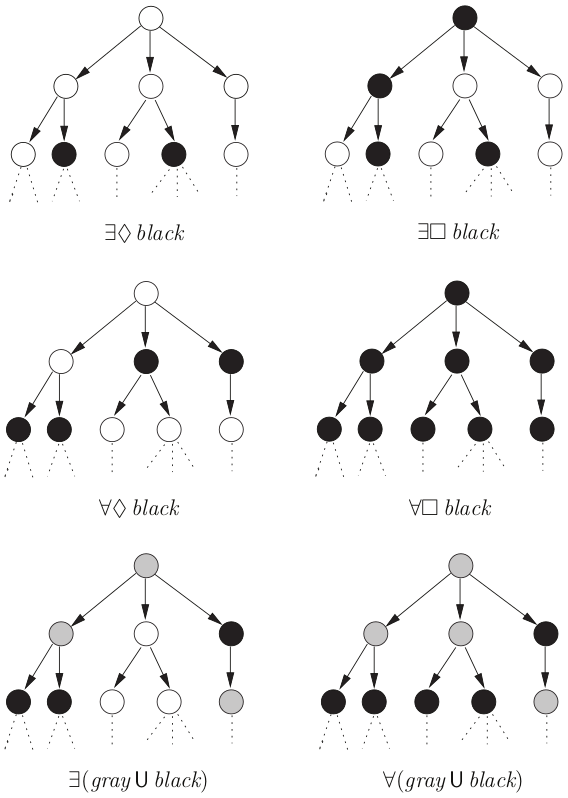
\includegraphics[width=0.8\textwidth]{ctl/imagenes/semanticaCTL.png}
\label{fig:semantica_CTL}
\end{center}
\end{minipage}
\end{figure}


\subsection{Propiedades}
En esta sección se muestran propiedades útiles para poder expresar todas las fórmulas
 de CTL utilizando un conjunto reducido y funcionalmente completo de conectivos.

\begin{itemize}
\item $\exists \lozenge \varphi = \exists (true \cup \varphi) $
\item $\forall \lozenge \varphi = \forall (true \cup \varphi) $
\item $\exists \square \varphi = \lnot \forall \lozenge \lnot \varphi $
\item $\forall \square \varphi = \lnot \exists \lozenge \lnot \varphi $
\item $\forall \bigcirc \varphi = \lnot \exists \bigcirc \lnot \varphi $
\item $\forall \lozenge \varphi = \lnot \exists \square \lnot \varphi $
\end{itemize}

Con estas propiedades es posible expresar cualquier propiedad en CTL mediante
 una fórmula CTL equivalente que sólo contenga el cuantificador existencial.


\subsection{CTL vs LTL}
Tanto CTL como LTL son lenguajes que permiten expresar muchas propiedades para un sistema.
 Pero son lógicas incompatibles entre sí. Esto quiere decir que existen fórmulas de CTL
 para las cuales no hay una equivalente en LTL y viceversa.

\begin{definicion}
Equivalencia entre fórmulas CTL y fórmulas LTL.\\
Una fórmula CTL $\varphi$ y una fórmula LTL $\psi$ son equivalentes si para todo
 sistema de transiciones $TS$:
\[ TS \models \varphi \text{ si y solo si } TS \models \psi \]
\end{definicion}

Un estado satisface una fórmula LTL $\varphi$ cuando todos los caminos a partir de
 este estado satisfacen $\varphi$.
De esto se puede observar que para obtener una fórmula LTL equivalente a una
 fórmula CTL dada basta con eliminar los cuantificacdores universales de la misma.
Más precisamente, dada una fórmula CTL, en caso de que exista un fórmula LTL
 equivalente, esta se obtiene eliminando los cuantificadores tanto universales
 como existenciales de la misma.
 